\documentclass{article}
\usepackage{import}
\subimport{../}{preamble}
\begin{document}

\section{Plasmons}
\label{sec:plasmons}

Plasmons are a direct solution of Maxwell's equations at the boundary between a dielectric and a metal. Despite existing on length scales from \SI{100}{nm} down to around \SI{1}{nm}, the high free electron density of metals mean energy levels still retain their characteristic continuous conduction bands and quantisation effects can be ignored.%
\footnote{A higher density of states means that energy levels are more closely spaced, hence metals with a large free electron density appear to have an energy continuum as opposed to discrete energy bands or levels at room temperature.}
Hence, classical theory is able to accurately describe physical phenomena until the characteristic length scale drops below $\sim$\SI{0.5}{nm} and a phenomenological approach using Maxwell's equations forms the basis of the mathematical description of plasmons.

\subsection{Electromagnetic Waves}
\label{sec:em_waves}

Maxwell's equations universally describe the classical, dynamical behaviour of \gls{em} waves, representing the foundations of electromagnetism. In their differential form they are given by,
\begin{subequations}
\begin{align}
	\nabla \cdot \vec{E} &= \frac{\rhotot}{\eps\epsfs}, \label{eq:maxwell1}\\
	\nabla \cdot \vec{B} &= 0, \label{eq:maxwell2}\\
	\nabla \times \vec{E} &= -\frac{\partial \vec{B}}{\partial t}, \label{eq:maxwell3}\\
	\nabla \times \vec{B} &= \mu\mu_0 \left( \vec{J} + \eps\epsfs \frac{\partial \vec{E}}{\partial t} \right), \label{eq:maxwell4}
\end{align}
\end{subequations}
where \gls{E} is the electric field, \gls{B} is the magnetic flux density, \gls{eps0} is the permittivity of free space, \gls{mu0} is the permeability of free space, \gls{rho_tot} is the (volume) charge density, \gls{J} is the current density and \gls{t} is time. The variables \gls{eps} and \gls{mu} are the relative permittivity and permeability, respectively, and describe the electromagnetic properties of the medium in which the fields exist. The \textit{electric displacement field} \gls{D} and the \textit{magnetic field} \gls{H} can be introduced to include material dependencies and describe macroscopic fields, which are defined by,
\begin{subequations}
\begin{align}
	\vec{D} &= \epsfs\vec{E} + \vec{P}, \label{eq:displacement_field}\\
	\vec{H} &= \frac{1}{\mu_0}\vec{B} + \vec{M}, \label{eq:magnetic_field}
\end{align}
\end{subequations}
where \gls{P} is the polarisation (dipole moment per unit volume) and \gls{M} the magnetisation. Equations \eqref{eq:maxwell1} and \eqref{eq:maxwell4} can then be redefined as,
\begin{subequations}
\begin{align}
	\nabla \cdot \vec{D} &= \rhoext, \label{eq:new_maxwell1}\\
	\nabla \times \vec{H} &= \Jext + \frac{\partial \vec{D}}{\partial t}, \label{eq:new_maxwell4}
\end{align}
\end{subequations}
to describe macroscopic \gls{em} fields within media. The charge and current densities now refer to only the external contributions, related to the internal contributions via $\rhotot=\rhoext+\rhoint$ and $\Jtot=\Jext+\Jint$.

The displacement field arises due to polarisation of a material in response to an applied field and is related to the internal charge density by $\nabla\cdot\vec{P}=\rhoint$. Conservation of charge means that $\nabla\cdot\vec{J}=\partial\rho/\partial t$, which requires that $\vec{J}=\partial\vec{P}/\partial t$ (a result also achievable by differentiating \eqref{eq:displacement_field}). The final equation of importance is the relationship between the electric field and the current density, given by,
\begin{equation}
	\vec{J} = \sigma\vec{E},
	\label{eq:current_density}
\end{equation}
where \gls{conductivity} is the conductivity. These few relations are sufficient to understand the behaviour of electromagnetic waves in media.

% Wave equation
Propagation of EM waves within a medium is governed by a wave equation relating both the spatial and temporal changes of a wave.
%In general, a wave equation describing a wave $\gls{wave_func}(x)$ along an axis \gls{x} in time $t$ is of the form,
%\begin{equation}
%	\frac{\partial^2 \psi}{\partial x^2} = \frac{1}{v^2} \frac{\partial^2 \psi}{\partial t^2},
%	\label{eq:form_wave_equation}
%\end{equation}
%where \gls{v} is the speed of the wave.
Combining \eqref{eq:maxwell3} and \eqref{eq:maxwell4} leads to the general wave equation for \gls{em} waves in the time domain,%
\footnote{Derived using $\nabla \times \nabla \times \vec{E} = \nabla(\nabla\cdot\vec{E}) - \nabla^2\vec{E}$}%
\begin{align}
	\nabla(\nabla\cdot\vec{E}) - \nabla^2\vec{E} &= -\eps\epsfs\mu\mu_0\frac{\partial^2\vec{E}}{\partial t^2} - \mu\mu_0\gls{J},% \\
	%\nabla(\nabla\cdot\gls{D}) - \nabla^2\gls{D} &= \frac{\partial^2\gls{D}}{\partial t^2} - \Jext,
	\label{eq:wave_equation}
\end{align}
describing the propagation of an \gls{em} wave in a given medium.
In the absence of both charge and current \eqref{eq:wave_equation} reduces to,
\begin{equation}
	\nabla^2\vec{E} = \eps\epsfs\mu\mu_0\frac{\partial^2\vec{E}}{\partial t^2},
\end{equation}
describing a wave propagating in both space and time with a velocity $\gls{v}=1/\sqrt{\epsfs\eps\mu_0\mu}$. In free space ($\eps=\mu=1$) this is the speed of light $\gls{c}=1/\sqrt{\epsfs\mu_0}$, with light slowed when in media to $v=c/\refind$ by a factor $\gls{refractive_index}=\sqrt{\eps\mu}$ known as the refractive index.

% Relate to plasmons
In general \eps\ is a complex quantity, $\eps=\eps_1+i\eps_2$, and depends on the frequency of the EM wave, \gls{omega}. Plasmons are a phenomenon resulting from this frequency dependence in metallic materials. The relative permittivity is therefore denoted \dielectric\ and is referred to as the material's dielectric function from this point onwards. The concept of a plasmon can be discerned through this function alone. Equations are therefore simplified by setting $\mu=1$ and removing any magnetic contributions.
% refractive index
Since \dielectric\ is a complex parameter with components $\eps_1+i\eps_2$, the complex refractive can be expressed as $\refind=\sqrt{\dielectric}=n+i\kappa$, where $n$ is the real part causing refraction and $\kappa$ is the loss coefficient determining absorption in the medium. The complex refractive index and the dielectric function are then related via $\eps_1=n^2-\kappa^2$ and $\eps_2 = 2n\kappa$.

The dispersive properties of a material are found by solving \eqref{eq:wave_equation} with $\eps=\dielectric$, describing the behaviour of a wave propagating through a non-magnetic, dielectric medium. For a propagating \gls{em} wave with frequency $\omega$ and wave vector \gls{wavevector} in space \gls{rv} of the form,
\begin{equation}
	\vec{E} = \gls{E0} \e^{i(\wv \cdot \vec{r} - \omega t)},
	\label{eq:wave}
\end{equation}
\eqref{eq:wave_equation} can be expressed in the frequency (Fourier) domain as,%
\footnote{Derived using the identities $\nabla \times \nabla \times \vec{E} = \nabla(\nabla\cdot\vec{E}) - \nabla^2\vec{E}$, $\nabla^2\vec{E}=-\wvm^2\vec{E}$ and $\partial^2\vec{E}/\partial t^2 = -\omega^2\vec{E}$ where $\nabla\cdot\vec{E}=0$}
\begin{equation}
	%\nabla(\nabla\cdot\vec{E}) - \nabla^2\vec{E} = -\eps(\wv, \omega) \frac{\omega^2}{c^2}\vec{E},
	\wv(\wv\cdot\vec{E}) - \wvm^2\vec{E} = -\eps(\wv, \omega) \frac{\omega^2}{c^2}\vec{E},
	\label{eq:fourier_wave_equation}
\end{equation}
where $\gls{wavevector_mag}=|\wv|$ is the magnitude of the wavevector. The variable $\gls{wavevector0} = \omega/c$ is sometimes used in \eqref{eq:fourier_wave_equation} when all quantities considered are wave vectors. From this equation the propagation behaviour of EM waves in media can be described.

Solutions to \eqref{eq:fourier_wave_equation} depend on the orientation of the wavevector with the field. Transverse wave solutions ($\wv\cdot\vec{E}=0$) yield the dispersion relation for light,
\begin{equation}
	\wvm = \sqrt{\eps(\wv, \omega)}\frac{\omega}{c}=\refind\wvz.
	\label{eq:light_dispersion}
\end{equation}
Inserting this into \eqref{eq:wave} gives a general solution for light propagating through a dielectric medium,
\begin{equation}
	\vec{E} = \gls{E0} \exp{\left({-\kappa\wvz r}\right)} \exp{\left[{i\omega\left(\frac{n}{c}r - t\right)}\right]}.
	\label{eq:gen_wave_solution}
\end{equation}
The real component of the refractive index $n$ slows the wave whereas the imaginary component corresponds to an exponential decay with characteristic length $1/\kappa$, representing loss within a medium.

Longitudinal wave solutions ($\wv\cdot\vec{E} = \wvm|\vec{E}|$) result in $\sqrt{\eps(\wv,\omega)}\omega/c = 0$, hence solutions only exists for $\eps(\wv, \omega)=0$. Both these conditions are important when describing plasmons in the bulk of a metal (only longitudinal plasmons are supported) and on the surface (both transverse and longitudinal plasmons supported).
%Furthermore, when considering the behaviour of \gls{em} waves at an interface between two different media the orientation of the fields with respect to the interface becomes important. Separate solutions exist depending on if a wave is considered \gls{tm} or \gls{te} (either only \vec{E} or \gls{H} has a component in the direction of propagation, respectively).%
%\footnote{\gls{te} and \gls{tm} are also known as $s$- and $p$-polarisations, respectively.}

Lastly, it should be noted that if the material dielectric properties in \eps\ are linear then $\vec{D}$ can be expressed in Fourier space as,\footnote{\color{red}Metals are linear in this regime so this expression holds}
\begin{equation}
	\gls{D}(\wv, \omega) = \epsfs\eps(\wv, \omega)\vec{E}(\wv, \omega).
	\label{eq:fourier_displacement_field}
\end{equation}
Combining \eqref{eq:fourier_displacement_field} with the differential of \eqref{eq:displacement_field}, \eqref{eq:current_density} and \eqref{eq:wave}%
\footnote{$\partial/\partial t \rightarrow -i\omega$ and $\vec{J}=\dot{\vec{D}}-\epsfs\dot{\vec{E}}=\epsfs\dot{\vec{E}}(\eps-1)=\sigma\vec{E}$}
yields a relation between a material's conductivity and it's dielectric function,
\begin{equation}
	\eps(\wv, \omega) = 1 + \frac{i\sigma(\wv, \omega)}{\epsfs\omega}.
	\label{eq:dielectric_conductivity}
\end{equation}
Both quantities are able to describe the same physics from a different perspective.%
\footnote{Choice of which variable to use is a matter of convenience and tradition. Either can be used to equally describe the electromagnetic response of a material. The conductivity is typically used to describe lower frequency phenomena while the dielectric function is used at higher frequencies.}
Since \real{\eps} is related to both \imag{\sigma} and \real{\refind}, \real{\sigma} must therefore be related to $\kappa=\imag{\refind}$ and the attenuation of waves inside media. A large conductivity in a material therefore corresponds to large transmission losses with decay attributed to energy transfer to move electrons at the surface of the material. Furthermore, the relation between \dielectric\ and $\sigma$ becomes important when considering points of conductance in a plasmonic system and that plasmons exist as an oscillating current.

% Lead into the optical properties of metals
Using the framework outlined so far the optical properties of metals can be deduced along with the existence of plasmons. The discussion begins with the Drude model for the optical response of metals \cite{drude1900}, which is used to first predict the behaviour of plasmons. From there the distinction can be made between plasmons within the volume of a metal and those confined to the surface, which are of most interest in plasmonics.

\subsection{Bulk Plasmons and the Optical Properties of Metals}

% work on this paragraph
Before studying the concept of a surface plasmon it is important to understand the optical properties of metals as bulk materials. The optical properties of a metal are dominated by the response of nearly-free electrons delocalised from the positive nuclei background. When light is incident on a metal, nearly free electrons at the surface respond to the field and are displaced in the opposite direction (since $\gls{F}=-e\vec{E}$). The field of the induced charge distribution cancels the electric field inside the metal. An \gls{em} wave impinging on a metal is internally screened{\color{red}, and therefore externally reflected,%
\footnote{Light excites electrons into a higher energetic state leading to re-emission upon decaying back to the ground state, or from a different point of view, the prevention of light from entering the metal means the incident field must be reflected.}
} through the displacement of free electrons inside the metal surface. The strong reflectance gives metals their shiny appearance. This behaviour originates from \eqref{eq:dielectric_conductivity}, where a high conductivity reduces the field penetration inside the metal. The exponential decay of the wave into the metal, shown in \eqref{eq:gen_wave_solution}, is characterised by the skin depth $\gls{skin_depth} = c/2\omega\kappa$, the point at which the field has decayed by $1/2\e$ of its original value.%
\footnote{The skin depth is defined using $1/2\e$ rather than $1/\e$ to consider power instead of field.}
Light transmission through a metal becomes heavily attenuated once its thickness becomes greater than \skindepth. The small values of \skindepth\ exhibited by metals means that they fall within the \textit{perfect conductor} approximation (zero internal field).

A metal starts to show a more ``dielectric-like" behaviour when the frequency of incoming light is high enough that the inertia of the electrons means they cannot respond instantaneously, preventing screening and thus transmitting the incident light. Such effects begin to be seen in the visible region of the \gls{em} spectrum in the case of noble metals. Fields increasingly penetrate the metal up until \gls{uv} photon energies, at which point most metals become transparent. This is known as the \textit{ultraviolet transparency}.

% Defining the dielectric function of a metal and discerning the plasma frequency (volume plasmons)
Since the dominating cause of these effects stems almost exclusively from nearly free electrons, as opposed to bound electrons,%
\footnote{Optical properties derived from bound electrons are described by a Lorentz oscillator model.}
the optical properties of metals can be classically described by the Drude model \cite{drude1900}. This model describes the motion of a free electron gas in response to an applied field. The equation of motion for a single electron in a time-varying applied field is given by,
\begin{equation}
	m\ddot{\gls{xv}}(t) + m\gamma \dot{\gls{xv}}(t) = -e\vec{E_x}(t),
\end{equation}
where \gls{m} is its effective optical mass and $\gls{gamma} = 1/\tau$ is the electron collision frequency, the inverse of the relaxation time, \gls{tau}. Using an effective optical mass as opposed to the actual electron mass incorporates band structure effects into the model. The electron collision frequency amounts to an effective coefficient of damping as in a mechanical oscillator. Inserting a harmonic driving field and assuming a similar oscillatory behaviour in the free electron displacement ($\vec{x} = \vec{x_0}\e^{-i\omega t}$) leads to a solution,
\begin{equation}
	\vec{x}(t) = \frac{e}{m(\omega^2 + i\gamma\omega)}\vec{E}(t).
	\label{eq:x_solution}
\end{equation}
There is a resulting polarisation $\vec{P}=-ne\vec{x}$ induced in the free electron gas, where \gls{n} is the density of electrons. The resulting displacement field, obtained by substituting \eqref{eq:x_solution} into \eqref{eq:fourier_displacement_field}%
\footnote{Derived from $\vec{D}=\epsfs\vec{E} + \vec{P} = \epsfs\vec{E} - [ne^2/m(\omega^2 + i\gamma\omega)]\vec{E} = \epsfs\eps(\omega)\vec{E}$}
, defines the dielectric function of a metal,
\begin{equation}
	\eps(\omega) = 1 - \frac{\omegap[2]}{\omega^2 + i\gamma\omega},
\end{equation}
where \gls{omega_p} is the plasma frequency of the metal, given by,
\begin{equation}
	\omegap[2] = \frac{ne^2}{\varepsilon_0 m}.
	\label{eq:plasma_frequency}
\end{equation}
The optical properties of a metal can be discerned from the real and imaginary components of \dielectric, given by,
\begin{subequations}
	\begin{align}
	\real{\dielectric} = \eps_1(\omega) &= 1 - \frac{\omegap[2]\tau^2}{1+\omega^2\tau^2},\\
	\imag{\dielectric} = \eps_2(\omega) &= \frac{\omegap[2]\tau}{\omega(1+\omega^2\tau^2)}.
	\end{align}
\end{subequations}
The plasma frequency defines the point at which the metal transitions into a dielectric. For $\omega<\omegap$, $\real{\eps(\omega<\omegap)} < 0$ and a free electron gas remains metallic in character, with electrons moving to oppose an incident field. Once $\omega > \omegap$ the free electron gas, limited by inertia, cannot respond fast enough to the field and the metal becomes dielectric in character.
% approximations to remove damping
For an ideal free electron gas with negligible damping the simplified expression,
\begin{equation}
	\dielectric = 1 - \frac{\omegap[2]}{\omega^2},
	\label{eq:dielectric_approx}
\end{equation}
is often used. This is the often the case for optical frequencies close to \omegap\ where the imaginary component of \dielectric, dominated by $\omega\tau\gg 1$, becomes negligible. In reality, however, interband transitions in real metals increase \imag{\dielectric}.
The expression for the dielectric function can be modified to account for interband absorption caused by bound electrons by the inclusion of a constant $\eps_\infty$. The dielectric function then has the form,
\begin{equation}
	\dielectric = \eps_\infty - \frac{\omegap[2]}{\omega^2 + i\gamma\omega}.
	\label{eq:dielectric_function}
\end{equation}

\begin{figure}[bt]
\centering
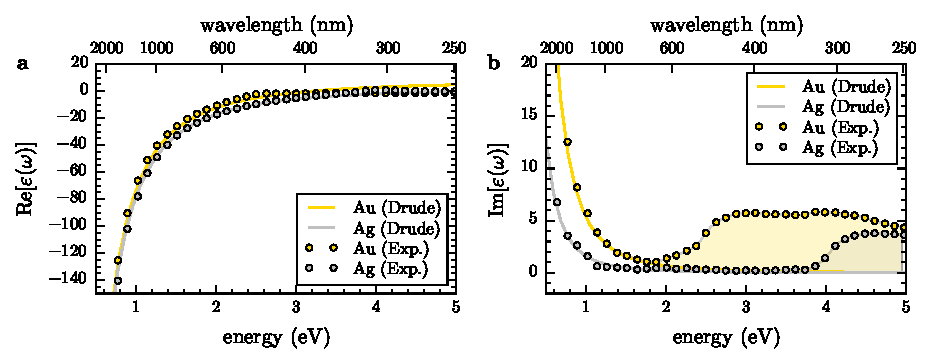
\includegraphics{figures/dielectric_function}
\caption[Plot of the dielectric function, given by the Drude model, for Au and Ag compared with empirical data]{\textbf{Plot of the dielectric function, given by the Drude model, for Au and Ag compared with empirical data.} \dielectric\ is calculated using \eqref{eq:dielectric_function}. The plasma frequency is calculated using \eqref{eq:plasma_frequency}. The parameters of the curves are $n=\SI{5.90e28}{\per\metre\cubed}$, $m=\SI{9.11e-31}{kg}$, $\gamma=1/\tau=1/\SI{1e-14}{s}$ and $\eps_\infty = 8$ for Au and $n=\SI{5.86e28}{\per\metre\cubed}$, $m=\SI{9.11e-31}{kg}$, $\gamma=1/\tau=1/\SI{3e-15}{s}$ and $\eps_\infty = 3$ for Ag. Empirical data (Johnson and Christy, 1972 \cite{johnson1972optical}) is shown for comparison to illustrate the importance of interband transitions. Differences between the Drude model (solid lines) and experimental results (circles) are caused by interband transitions not included in the basic Drude formalism.}
\label{fig:dielectric_function}
\end{figure}

A plot of \eqref{eq:dielectric_function} is shown in \figurename~\ref{fig:dielectric_function} , along with empirical data, illustrating both why noble metals exhibit high quality, visible spectrum (400--\SI{700}{nm}, 1.5--\SI{3}{eV}) plasmonics, as well as the failings of the Drude model. Noble metals have $\real{\dielectric}<0$ and small \imag{\dielectric} in the visible region, hence behave very similarly to an ideal free electron gas. The Drude model fails at higher energies as interband transitions are not included in the basic model. These transitions increase the absorption ($\propto\imag{\dielectric}$) and are significant for $\lambda < \SI{500}{nm}$ in Au and $\lambda<\SI{300}{nm}$ in Ag. A measure of the quality of a metal can de determined from its quality factor $\gls{Q} = \left|\real{\eps}/\imag{\eps}\right|$. The high $Q$ of noble metals in the visible regions means they can easily respond to an incident field and screen it, behaving metallically. %Interband transitions lead to a reduction in $Q$ at higher energies therefore preventing the large resonances associated with high quality plasmonic materials.
%Lorentz oscillator terms $m\omega_0i^2x$, where $\omega_0i$ are the natural frequencies of bound electron transitions, can be included in the initial equation of motion to account for such transitions.

\begin{figure}[bt]
\centering
\fontsize{10pt}{1em}\selectfont
\subimport{./figures/}{bulk_charge_displacement.pdf_tex}
\caption[Charge displacement of a free electron gas under an applied field]{\textbf{Charge displacement of a free electron gas under an applied field.} The optical electric field displaces the electrons leaving behind the positive cores. The slab becomes polarised with opposing surface charge densities $\sigma$. The charge oscillations resonate when the field frequency is \omegap.}
\label{fig:bulk_charge_displacement}
\end{figure}

The plasma frequency \omegap\ in \dielectric\ not only describes a metal-to-dielectric transition but also dictates the frequency of the collective longitudinal mode of oscillation. By substituting \eqref{eq:dielectric_approx} into the dispersion relations for transverse and longitudinal waves it is clear that transverse waves are only supported if $\omega>\omegap$ with a dispersion $\omega^2=\omegap[2]+\wvm^2c^2$. However, a collective longitudinal oscillation is allowed at $\omega=\omegap$ since $\dielectric=0$ in the absence of damping. In this case the free electron gas is displaced from the ionic core background a distance \gls{u} due to the applied field to form surface charge densities $\gls{sigma} = \pm neu$ (\figurename~\ref{fig:bulk_charge_displacement}). The resulting depolarisation field%
\footnote{Gauss' law $\int \vec{E}\cdot d\vec{A} = Q/\epsfs=\sigma A/\epsfs$, hence $E=\sigma/\epsfs$. Alternatively $D=0=\epsfs\vec{E}+\vec{P}$ therefore $\vec{E}=-\vec{P}/\epsfs=-ne\vec{u}/\epsfs$.}
is $E = neu/\epsfs$ and the motion of the free electrons is defined by,
\begin{equation}
	nm\ddot{u} = -neE = -\frac{n^2e^2u}{\epsfs}.
\end{equation}
Simplifying this relation leads to,
\begin{equation}
	\ddot{u}+\omegap[2] u=0,
\end{equation}
hence \omegap\ is considered the natural frequency of the system and the electrons resonate when driven at $\omega=\omegap$. This is known as the bulk or \emph{volume plasmon}. Since this is a longitudinal oscillation, however, light cannot couple with it. For this reason, volume plasmons cannot be excited and measured by means of optical techniques but require other experimental methods (e.g.\ \gls{eels} \cite{egerton2011electron}). Optical plasmonic phenomena must therefore be a result of a different kind of plasmon. % could cite koh2009

\subsection{Surface Plasmons}
% EELS of LSPs nelayah2007, koh2009, duan2012

\Glspl{sp}, unlike bulk plasmons, are collective oscillations of conduction electrons tightly confined to the surface of the metal. As stated previously, light at an interface is not necessarily restricted by the diffraction limit. The maximum magnitude of the wavevector is set by $\wvz=2\pi/\lambda$ with individual components restricted by $\wvm = \sqrt{\wvm_x^2 + \wvm_y^2 + \wvm_z^2}$. Consider \eqref{eq:light_dispersion} in the form,
\begin{equation}
	\wvm_x^2 = \refind^2 \wvz^2 - \wvm_y^2 - \wvm_z^2.
\end{equation}
If a wave propagates freely in all three dimensions then it remains diffraction limited and the propagation constant $\wvm_x < \refind\wvz$. However if one or more of its wavevector components become imaginary ($\wvm_{y,z}^2 < 0$) then it becomes possible that $\wvm_x > \refind\wvz$. This behaviour can occur at an interface, where surface waves take on evanescent character in the $z$-direction whilst propagating in the $xy$ plane.%
\footnote{Evanescent meaning imaginary $\wvm_z$ therefore exponentially decaying amplitude in the $z$-direction.}
By coupling light into surface waves the diffraction limit can be beaten. Waves of frequency $\omega$ can acquire wavelengths many times smaller than their excitation wavelength. The \gls{sp} is one such case of this phenomenon and occurs at metal-dielectric interfaces. % Are there other such cases.
Unlike in a bulk metal, electrons displaced by an applied field at the surface of a metal feel a restoring force due to the positive nuclei background. Transverse fields impinging on the metal surface at an angle are then able to manipulate the electron motion. \Glspl{sp} can therefore be excited by light as well as by the longitudinal waves needed to excite bulk plasmons, forming polariton quasiparticles under strong coupling with photons.%
\footnote{Polaritons are the name given to quanta or quasiparticles of light-matter interactions. Strong coupling describes the point at which a quasiparticle is no longer distinguishable between its two constituent components.}
This optical excitation is known as the \gls{spp} and, as a result of it being optically accessible, is one of the most commonly studied plasmonic phenomenons.

\subsubsection{Surface Plasmon Polaritons}

\begin{figure}[bt]
\fontsize{10pt}{1em}\selectfont
\def\svgwidth{0.6\textwidth}
\subimport{./figures/}{spp_diagram.pdf_tex}
\caption[Diagram of a surface plasmon polariton (SPP)]{\textbf{Diagram of a surface plasmon polariton (SPP).} TM surface electron density waves (surface plasmons) couple with an evanescent wave originating from an EM wave to form a SPP. The SPP remains confined to the interface but can propagate across the surface.}
\label{fig:spp_diagram}
\end{figure}

A \gls{spp} is a propagating \gls{tm} wave confined to the surface of a metal - the bound state between a photon and a \gls{sp}.
The \gls{tm} nature of the wave indicates that \vec{E} has a component traversing across the interface as shown in the diagram of a SPP in \figurename~\ref{fig:spp_diagram}. No such solution exists for \gls{te} surfaces waves (i.e. a component of \vec{H} passing through the interface).%
\footnote{\gls{te} and \gls{tm} are also known as $s$- and $p$-polarisations, respectively.}
While confined in two dimensions to the planar boundary between a metal and a dielectric, the \gls{spp} can either propagate or become stationary as a result of interference {\color{red}with itself or other plasmons}. The latter stationary form of the \gls{spp} is similar to the localised surface plasmons, described later.

The \gls{spp} itself is described through its dispersion. As a \gls{tm} wave propagating in the $x$-direction along a metal/dielectric interface, it has a spatial field profile in a space \vec{x} given by $\vec{E}(\vec{x}) = \vec{E}(z)\e^{i\beta x}$ where $\beta=\wvm_x$ is the propagation constant. The magnetic field in this configuration is then $\vec{H}(\vec{x}) = \vec{H}(y)e^{i\beta x}$. The behaviour of such a wave in \eqref{eq:fourier_wave_equation} is described by,
\begin{subequations}
\begin{align}
	\frac{\partial^2\vec{E}(z)}{\partial z^2} + (\wvz^2\eps - \beta^2)\vec{E} &= 0,\\
	\frac{\partial^2\vec{H}(y)}{\partial y^2} + (\wvz^2\eps - \beta^2)\vec{H} &= 0.
\end{align}
\end{subequations}
Both equations can be related using \eqref{eq:maxwell3} and \eqref{eq:maxwell4}. Assuming a \gls{tm} wave ($\partial E_y/\partial z = 0$, $\partial H_z/\partial z = 0$), propagating only in the $x$-direction with symmetry in $y$-direction, results in the field relations,
\begin{subequations}
\begin{align}
	E_x &= -i\frac{1}{\omega\epsfs\eps}\frac{\partial H_y}{\partial z},\\
	E_z &= -\frac{\beta}{\omega\epsfs\eps}H_y.
\end{align}
\end{subequations}
In this instance the \gls{tm} wave equation, and requirement for evanescent decay in the $z$-direction, mean that $H_y = A_d\e^{i\beta x}\e^{-\wvdi z}$ for $z>0$ (in the dielectric) and $H_y = A_m\e^{i\beta x}\e^{\wvmet z}$ for $z<0$ (in the metal). The components of the electric field can therefore be expressed as,
\begin{subequations}
\begin{align}
	E_x(z) &= iA_d\frac{1}{\omega\epsfs\epsdi}\wvdi\e^{i\beta x}\e^{-\wvdi z},\\
	E_z(z) &= -A_d\frac{\beta}{\omega\epsfs\epsdi}\e^{i\beta x}\e^{-\wvdi z},
\end{align}
\end{subequations}
inside the dielectric and,
\begin{subequations}
\begin{align}
	E_x(z) &= -iA_m\frac{1}{\omega\epsfs\epsmet}\wvmet\e^{i\beta x}\e^{\wvmet z},\\
	E_z(z) &= -A_m\frac{\beta}{\omega\epsfs\epsmet}\e^{i\beta x}\e^{\wvmet z},
\end{align}
\end{subequations}
inside the metal, where $\epsmet=\dielectric$ in the previously used notation. Continuity across the boundary ($z=0$) dictates that $A_d=A_m$ and yields the relation,
\begin{equation}
	\frac{\wvmet}{\wvdi} = -\frac{\epsmet}{\epsdi},
	\label{eq:wavevector_ratio}
\end{equation}
hence the ratio between wavevectors inside and outside of the metal depends on the relative change in dielectric constant across the boundary. It is this continuity relation that allows for the existence of \glspl{spp} in the \gls{tm} configuration.%
\footnote{No such continuity equation exists for TE waves, hence SPPs cannot exist in this configuration.}
To determine the \gls{spp} propagation constant $\beta$ a further relation is needed to fix the wave vectors in a given medium with respect to the dielectric constant. Using the expression for $H_y$ in the wave equation \eqref{eq:fourier_wave_equation} yields a set of relations,
\begin{subequations}
\begin{align}
	\wvmet^2 = \beta^2 - \wvz^2\epsmet,\\
	\wvdi^2 = \beta^2 - \wvz^2\epsdi,
\end{align}
\end{subequations}
which, when combined with \eqref{eq:wavevector_ratio}, fully describe the fields around the interface. The propagation constant is then given by,
\begin{equation}
	\beta = \frac{\omega}{c}\sqrt{\frac{\epsdi\dielectric}{\epsdi + \dielectric}}.
	\label{eq:spp_dispersion}
\end{equation}
\begin{figure}[bt]
\centering
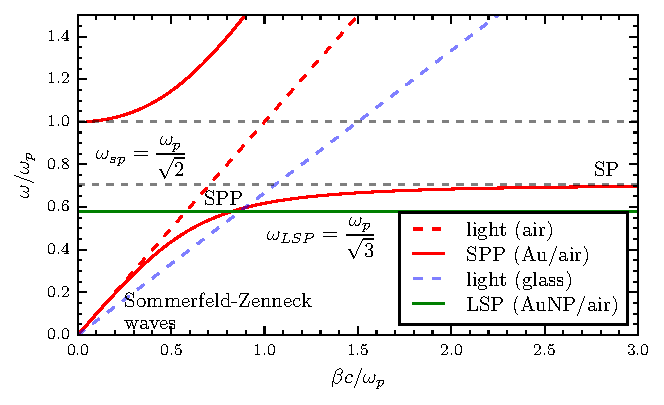
\includegraphics{figures/spp_dispersion}
\caption[Plasmon dispersion relations for the SPP and LSP]{\textbf{Plasmon dispersion relations for the SPP and LSP.} The dashed lines indicate the dispersion of light in both glass and air (vacuum) along with the surface plasmon frequency. SPPs can be described as photon-like or plasmon-like depending on their point of excitation. SPPs excited with large \wvm\ and $\omega\approx\omega_{SPP}$ are considered plasmon-like while SPPs with low \wvm\ are considered more photon-like. These have been known as Sommerfeld-Zenneck surface waves \cite{kittel1976introduction}.}
\label{fig:spp_dispersion}
\end{figure}
This is the dispersion relation for a \gls{spp}, as is shown in \figurename~\ref{fig:spp_dispersion} along with the dispersion of light for both air and glass mediums.

% Excitation of SPPs
From the dispersion curve it is clear that \glspl{spp} cannot couple with light within the same medium as their dispersion curves do not cross. However, light from within a higher refractive index medium such as glass can generate evanescent waves and excite \glspl{spp} on a nearby metal/air interface. This method of coupling photons with surface plasmons, depending on the specific prism arrangement, is known as the Kretschmann (prism-metal-dielectric) or Otto (prism-dielectric-metal) configuration \cite{otto1968, kretschmann1971}. Since a diffraction grating may also impart momentum onto a photon ($\wvm_x \rightarrow \wvm_x + n\pi$) a metallic grating can launch \glspl{spp} along a planar metal-dielectric interface. This phenomenon was first observed in 1902 by Wood, dubbed as Wood's anomaly \cite{wood1902}, and only explained via surface waves many years later \cite{fano1941}.

% Plasmon property: nm-scale wavelength with visible frequency
Closer inspection of the curve highlights one of the major features of a plasmon. While \glspl{spp} retain the frequency of the excitation field, their wavelength is considerably smaller than the diffraction-limited wavelength of light.
% photon-like vs plasmon-like
Depending on where on the curve the \gls{spp} lies it can be considered to be either more photon-like or more plasmon-like. For small $\beta\approx\wvz$ the \gls{spp} is similar to light grazing the interface (Sommerfeld-Zenneck waves)%
\footnote{Sommerfeld-Zenneck waves are surface waves that appear throughout mechanics and electromagnetism that are confined to the interface between two different mediums.}
whereas \glspl{spp} with large \wvm\ become more plasmon-like and their frequency saturates at the surface plasmon frequency,
\begin{equation}
	\omegasp = \frac{\omegap}{\sqrt{1+\epsdi}}.
\end{equation}
At this point the \gls{spp} can be considered electrostatic and becomes a \gls{sp}. To some extent, \glspl{sp} confined to a finite, continuous, non-planar surface, defining a \gls{np}, can be considered to be the basis for a \gls{lsp} {\color{red}or \gls{lspp}}.

\subsubsection{Localised Surface Plasmons}

% Localised Surface Plasmons
\Glspl{lsp} are collective oscillations of conduction electrons confined within a fixed sub-wavelength spatial extent. These can occur on any nanoscale curved surface but the effects are strongest, and most well-documented, on the surface of a \gls{mnp}. Free electrons are displaced from the nuclei in response to an applied field and form a surface charge distribution, polarising the particle. Coulomb interaction between the poles of the surface charge distribution results in a restoring force within the particle. This gives rise to a natural frequency of oscillation, leading to a \gls{spr} when driven harmonically at the correct frequency.
The particle geometry sets which multipolar surface charge distributions are supported, while its material properties and the dielectric properties of the surrounding medium set the restoring force. Each different multipolar charge distribution is therefore considered to be a unique \gls{lsp} mode, identifiable by its \gls{spr} \cite{murray2007}.
%This bears some similarity with the slab of free electron gas supporting longitudinal volume plasmons, shown in \figurename~\ref{fig:bulk_charge_displacement}, except that the sub-wavelength geometry modifies the restoring force and allows transverse modes of oscillation. The plasma frequency in \glspl{lsp} is then rescaled by a factor depending on the geometry of each \gls{lsp} mode. %In this sense, \glspl{lsp} can be considered geometrical resonances of the nanostructure. % Not strictly true as geometrical resonances can occur in dielectrics

\begin{figure}[bt]
\centering
\fontsize{10pt}{1em}\selectfont
\def\svgwidth{0.35\textwidth}
\subimport{./figures/}{sphere_plasmon.pdf_tex}
~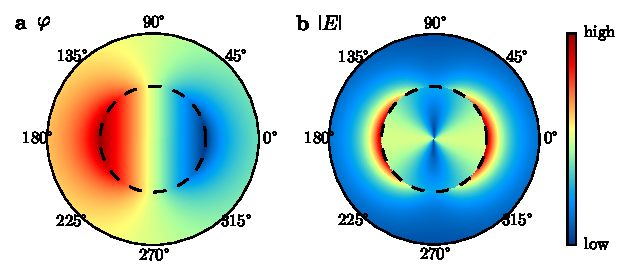
\includegraphics[width=0.59\textwidth]{figures/spherical_np_dipole_lsp}
\caption[A spherical metallic particle in an applied electric field]{\textbf{A spherical metallic particle in an applied electric field.} The sphere is assumed to in the quasistatic regime ($a\ll\lambda$). The aura around the particle indicates the phase of the free electron oscillations in the plasmon. Calculations of (a) the potential and (b) the magnitude of the electric field for a spherical nanoparticle on resonance ($\dielectric=-2\epsdi$).}
\label{fig:sphere_plasmon}
\end{figure}

The simplest form of a \gls{lsp} is the dipole resonance of a spherical \gls{mnp}. Assuming the sphere radius $\gls{a}\ll\lambda$ (the wavelength of light), the particle is considered to be in the quasistatic regime, where electrons move instantaneously in response to the incident field and its phase is ignored. Electrostatics, rather than electrodynamics, then becomes applicable to solve the problem. The electrostatic potential, \gls{potential}, of the system is described by the Laplace equation, $\nabla^2\pot=0$, with a general solution in a spherical geometry of the form \cite{maier2007plasmonics},
\begin{equation}
	\pot_{l,m_l}(r,\theta,\phi) = \sum_{l=0}^{l=\infty} \sum_{m_l=-l}^l [ A_lr^l + B_lr^{-(l+1)} ] P_l^m (\cos\theta) \e^{i m_l\phi},
\end{equation}
where \gls{l} is the degree of spherical harmonic and \gls{m_l} its projection, $A_l$ and $B_l$ are constants and $P_l^m(\cos\theta)$ are associated Legendre polynomials. For a sphere of radius $a$ and dielectric function \dielectric\ in a dielectric medium described by \epsdi\ the solution is fixed by the boundary conditions $\pot_{\mathrm{out}}\rightarrow-E_0z$ as $r\rightarrow\infty$ and $\left.\nabla\pot_{in}(r)\right|_{r=a}=\left.\nabla\pot_{out}(r)\right|_{r=a}$. This reduces to a solution \cite{jackson1999classical},
\begin{equation}
	\pot =
	\begin{dcases}
	-\frac{3\epsdi}{\dielectric + 2\epsdi} \vec{E_0}\cdot\vec{r} & r \leq a\text{ (inside)}, \\
	\left(-1 + \frac{\dielectric - \epsdi}{\dielectric + 2\epsdi} \frac{a^3}{r^3}\right) \vec{E_0}\cdot\vec{r} & r > a\text{ (outside)}.
	\end{dcases}
\end{equation}
For a metal sphere the potential (plotted in \figurename~\ref{fig:sphere_plasmon}a) describes an induced dipolar surface charge distribution. The description is simplified by defining the dipole moment,
\begin{equation}
	\vec{p} = \epsfs\epsdi\alpha\vec{E_0} = 4\pi\epsfs\epsdi a^3 \frac{\dielectric - \epsdi}{\dielectric + 2\epsdi} \vec{E_0},
\end{equation}
where the polarisability, \gls{alpha}, incorporates the frequency dependent behaviour and is defined as,
\begin{equation}
	\alpha(\omega) = 4\pi a^2 \frac{\dielectric - \epsdi}{\dielectric + 2\epsdi}.
	\label{eq:polarisability}
\end{equation}
The outside potential is then expressed as,
\begin{equation}
	%\Phi_{out} = -E_0r\cos{\theta} + \frac{\vec{p}\cdot\vec{r}}{4\pi\varepsilon_0\varepsilon_m r^3}.
	\pot_{out} = -\vec{E_0}\cdot\vec{r} + \frac{\vec{p}\cdot\vec{r}}{4\pi\epsfs\epsdi r^3}.
\end{equation}
This is simply the potential of an induced dipole superimposed onto the incident field. The electric field inside and outside of the sphere, calculated using $\vec{E}=-\nabla\pot$ and given by,
\begin{equation}
	\vec{E} =
	\begin{dcases}
	\frac{3\epsdi}{\dielectric+2\epsdi} \vec{E_0} & r \leq a\text{ (inside)}, \\
	\vec{E_0} + \frac{3\vec{n}(\vec{n}\cdot\vec{p}) - \vec{p}}{4\pi\epsfs\epsdi}\frac{1}{r^3} & r > a\text{ (outside)},
	\end{dcases}
	\label{eq:E_out}
\end{equation}
where $\vec{n}=\vec{r}/r$ is the radial unit vector, shows a similar phenomenon and is shown in \figurename~\ref{fig:sphere_plasmon}b.

Provided that the quasistatic approximation remains valid, the electrostatic result is simply multiplied with a harmonic time dependence to describe electrodynamic behaviour. An \gls{em} wave therefore induces a coherent, oscillating dipole moment $\vec{p}\e^{i\omega t}=\epsfs\epsdi\alpha\vec{E_0}\e^{i\omega t}$. The behaviour of electrons in the spherical \gls{mnp} at optical frequencies, described using the dielectric function \dielectric, is then simply incorporated into $\alpha(\omega)$. For a good metal $\real{\dielectric}<0$ and the denominator in \eqref{eq:polarisability} undergoes resonance%
\footnote{$\alpha\rightarrow-\infty$ when $\dielectric+2\epsdi\rightarrow0$}
at the Fr\"{o}hlich condition when,
\begin{equation}
	\real{\dielectric} = -2\epsdi. \label{eq:frohlich}
\end{equation}
This corresponds to excitation of a collective oscillation of conduction electrons on the surface of the sphere - the dipolar \gls{lsp}. Its magnitude in real metals is restricted by damping of the electron motion leading to a Lorentzian-shaped resonance band - the dipolar \gls{spr}. Its relationship with \epsdi\ means that the \gls{spr} can be tuned by varying the external dielectric medium. As seen in \eqref{eq:E_out}, the field from the induced dipole moment of the plasmon is superimposed onto the incident field leading to a resonant enhancement, both inside and outside the surface of the sphere. This is one of the fundamental properties of the plasmon, and one that is most exploited in sensing and sensor developments.

In the Drude model, with \dielectric\ given by \eqref{eq:dielectric_function}, the Fr\"{o}hlich condition is satisfied when,
\begin{equation}
	\omegalsp = \frac{\omegap}{\sqrt{1+2\epsdi}},
\end{equation}
which evaluates to $\omega = \omegap/\sqrt{3}$ for a \gls{mnp} in vacuum. As can be seen in \figurename~\ref{fig:spp_dispersion}, the flat dispersion of a \gls{lsp} mode means it crosses the light line at a single point. Light of the correct frequency therefore readily couples with \glspl{lsp} without the need for \gls{spp} momentum matching mechanisms.
% Spherical harmonics
In general, the optical spectrum of a \gls{mnp} can contain a number of multipolar plasmon modes for which the resonant frequencies are given by \cite{prodan2004},
\begin{equation}
	\omega_l = \omegap\sqrt{\frac{l}{\epsdi(l+1)+1}},
\end{equation}
where the degree of spherical harmonics $l$ denotes the charge distribution of a specific mode ($l=1$ for dipole, $l=2$ for quadrupole, etc.). However, these modes only exist outside of the quasistatic regime in larger \glspl{mnp} or more complex geometries.
% Link with noble metals
For nobles metals, such as Au and Ag, the fundamental $l=1$ mode occurs in the visible region of the \gls{em} spectrum ($\lambda=\SI{520}{nm}$ for Au and $\lambda=\SI{360}{nm}$ for Ag in vacuum or air \cite{maier2007plasmonics}, redshifted in the presence of other media \cite{sonnichsen2000}), leading to them often being the plasmonic metal of choice.
% geometry dependence
Additionally, the polarisability changes with \gls{np} geometry due to differing restoring forces acting on the surface charge distribution. Changes from a spherical shaped \gls{np} therefore lead to tuning of the \glspl{spr} across the visible spectrum. This geometrical dependence is well known \cite{krenn2000, mock2002, kuwata2003} and has been exploited in many applications over the past decade, e.g.\ \gls{ir} photothermal therapy \cite{huang2006, huang2008, huang2010gold}.

The larger the separation between opposing poles of surface charge, the weaker the restoring force. A larger particle, or similarly an elongated particle (a nanoellipsoid or nanorod), will therefore have lower energy resonances. Simple changes can be made to the theoretical (quasistatic) model to account for an ellipsoidal geometry, and thus somewhat understand the geometrical dependencies incorporated into the polarisability. Insertion of a geometrical correction to the polarisability leads to the definition \cite{maier2007plasmonics, noguez2007},
\begin{equation}
	\alpha_i(\omega) = 4\pi a_1a_2a_3\frac{\dielectric-\epsdi}{3\epsdi+3L_i(\dielectric-\epsdi)},
\end{equation}
where $i$ is the index of each anisotropic axis with a geometrical factor,
\begin{equation}
	L_i = \frac{a_1a_2a_3}{2}\int_0^\infty \frac{dq}{(a_i^2+q)\sqrt{(q+a_1^2)(q+a_2^2)(q+a_3^2)}}.
\end{equation}
The resonance condition along each axis then becomes,
\begin{equation}
	\real{\dielectric} = -\frac{1 - L_i}{L_i}\epsdi.
\end{equation}
By increasing the size of an axis, decreasing its associated geometrical factor, the resonance condition decreases from $\dielectric=-2\epsdi$, redshifting the \gls{spr}. The more elongated the particle becomes, the larger the redshift until the restoring force is weakened to the point that each lowest-order antenna \gls{spr} no longer exists.

\subsubsection{Optical Observation of Surface Plasmon Resonances}

Depending on the microscopic dipole moment of excited plasmons, their fields can be radiative and hence macroscopically observable. This depends on the geometry of the plasmons time-varying charge distribution. Antenna-like dipolar plasmons bear similarity with the Hertzian dipole, an infinitesimal oscillating current source which both absorbs and radiates EM waves. The relationship between the current, $\vec{I}(t)$, carried by the dipole of length $d$ and the radiative electric field around it is given by \cite{grant2013electromagnetism},
\begin{equation}
	\vec{E} = \frac{ik\vec{I}d\eta_o}{4\pi r} \e^{-ikr} \left[ \hat{r} \left( \frac{1}{ikr} + \frac{1}{(ikr)^2} \right) 2\cos\theta + \hat{\theta} \left( 1 + \frac{1}{ikr} + \frac{1}{(ikr)^2} \right) \sin\theta \right],
\end{equation}
The radial behaviour of the electric field around an object can be split into three distinct regimes - the \emph{near-field}, Fresnel regime and the \emph{far-field} or Fraunhofer regime. At short distances the $(\wvm r)^{-2}$ term dominates to form the near-field but quickly falls off with increasing distance. The remaining $(\wvm r)^{-1}$ term defines the far-field. The Fresnel regime forms the intermediate stage between the two. The boundary between the near-field and the far-field is defined as the point at which $\wvm r=1$ where $r = \lambda/2\pi$ (hence why sub-wavelength optics deals with the near-field).

Plasmons similarly have the ability to both resonantly absorb and scatter incident fields. The absorbance and scattering cross sections determining interaction with a spherical \gls{mnp} are given by \cite{bohren2008absorption},
\begin{subequations}
\begin{align}
	\gls{sigma_scat} &= \frac{\wvm^4}{6\pi} |\alpha|^2 = \frac{8\pi}{3}\wvm^4a^6 \left| \frac{\dielectric - \epsdi}{\dielectric + 2\epsdi} \right|^2, \\
	\gls{sigma_abs} &= \wvm\imag{\alpha} = 4\pi \wvm a^3 \imag{ \frac{\dielectric - \epsdi}{\dielectric + 2\epsdi} }.
\end{align}
\end{subequations}
Since $\sigma_{\mathrm{scat}} \propto V^2$ and $\sigma_{\mathrm{abs}} \propto V$, absorption dominates in smaller particles whilst larger particles scatter more strongly. The extinction cross section, commonly used in spectroscopy, can be calculated using $\gls{sigma_ext}=\sigma_{\mathrm{scat}}+\sigma_{\mathrm{abs}}$. The size of each cross-section, i.e.\ the spatial extent over which light interacts with the \gls{mnp}, depends on $\alpha$ and is increased on resonance. Hence, \glspl{mnp} optically appear strongly coloured and much larger than they actually are.%
\footnote{Consider that $\sigma_{\mathrm{scat}}$ for a AuNP is enhanced $100\times$ on resonance, meaning it's area cross-section is $\sqrt{100/\pi}= 6\times$ wider than it's radius, hence why a \SI{50}{nm} AuNP looks like a \SI{300}{nm} green sphere when imaged.}

For example, when on resonance with the dipolar \gls{lsp}, both cross sections are enhanced by the polarisability resonance from \orderof{$a\sim\SI{50}{nm}$} to \orderof{\SI{500}{nm}}. The increased size of the cross-section is comparable to the wavelength of light, meaning \glspl{lsp} efficiently couple with photons in the far-field. The \gls{lsp} mediates energy transfer between the near-field and the far-field and acts to match the electromagnetic modes of nanoscale absorbers/emitters, such as phonons (Raman) and radiative energy levels (quantum emitters, fluorescence), with those of a diffraction-limited photonic mode via an oscillating charge density \cite{berweger2012}. A plasmonic \gls{np} is often therefore described as an \textit{optical antenna} in a similar manner to a device that converts between radio waves and an electrical current is named a radio antenna \cite{bharadwaj2009, novotny2011}. \Gls{lsp} modes which readily couple with the far-field are then sometimes referred to as \emph{antenna modes} and become important when designing resonant structures for specific sensing applications.

\begin{figure}[bt]
\centering
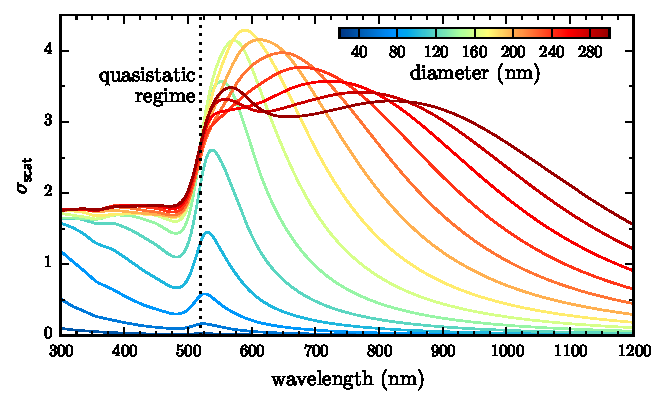
\includegraphics{figures/mie_scattering}
\caption[Mie scattering cross-sections for AuNPs of increasing diameter]{\textbf{Mie scattering cross-sections for AuNPs of increasing diameter.} The \SI{520}{nm} resonance position of the dipolar LSP mode of a AuNP in the quasistatic approximation is indicated by the dotted line. The resonance stays at \SI{520}{nm} until $d>\SI{80}{nm}$ then redshifts. The emergence of higher order modes following a similar behaviour is seen once $d>\SI{100}{nm}$.}
\label{fig:mie_scattering}
\end{figure}

Whilst the quasistatic approach is useful to first demonstrate the field enhancing capabilities of a \gls{mnp}, the description breaks down once the size of the particle becomes closer to the excitation wavelength. Retardation effects between the field and the electrons mean that phase differences between the charge oscillations and the incident field become important. At this point Mie theory (electrodynamics) \cite{mie1908} is required to describe the spectral response of spherical \glspl{mnp}. Mie theory provides a more general description of the optical response of spherical \glspl{mnp}. Using this approach the spectrum of a \gls{mnp} can be decomposed into superimposed multipoles, alluding to the existence of higher order \gls{lsp} modes in larger \glspl{mnp}. The spectral response of spherical AuNPs of varying sizes is shown in \figurename~\ref{fig:mie_scattering}, demonstrating the redshift and broadening of lower order modes with increasing particle size and the excitation of higher order modes.
%Furthermore, from \figurename~\ref{fig:mie_scattering}, though the scattering cross-section given by Mie theory is significantly less than from the electrostatic result, the enhanced cross-section still remains relatively large in comparison. This again explains why diffraction-limited light efficiently couples well with metallic nanostructures. The increased cross sections acts as a means of mode-matching the similarly sized incident fields with the nanoscale geometry.

% Lead into plasmon coupling
To summarise, by utilising the particle material, geometry and polarisation anisotropy its \glspl{spr} can be tuned across the entire UV--NIR spectrum to tailor to individual applications. However, even when exciting on resonance, a single particle can only provide a relatively small field enhancement. An alternative approach to exploiting \glspl{lsp} is therefore to couple the fields of many plasmons together. Through coupling, the confined fields in nanometric-size gaps between \glspl{mnp} can be enhanced by many more orders of magnitudes.

\end{document}